\section{Results and Discussion}

\subsection{Elementary Perceptual Tasks}

some are good and some are bad.. why?

\begin{figure*}[h]
	  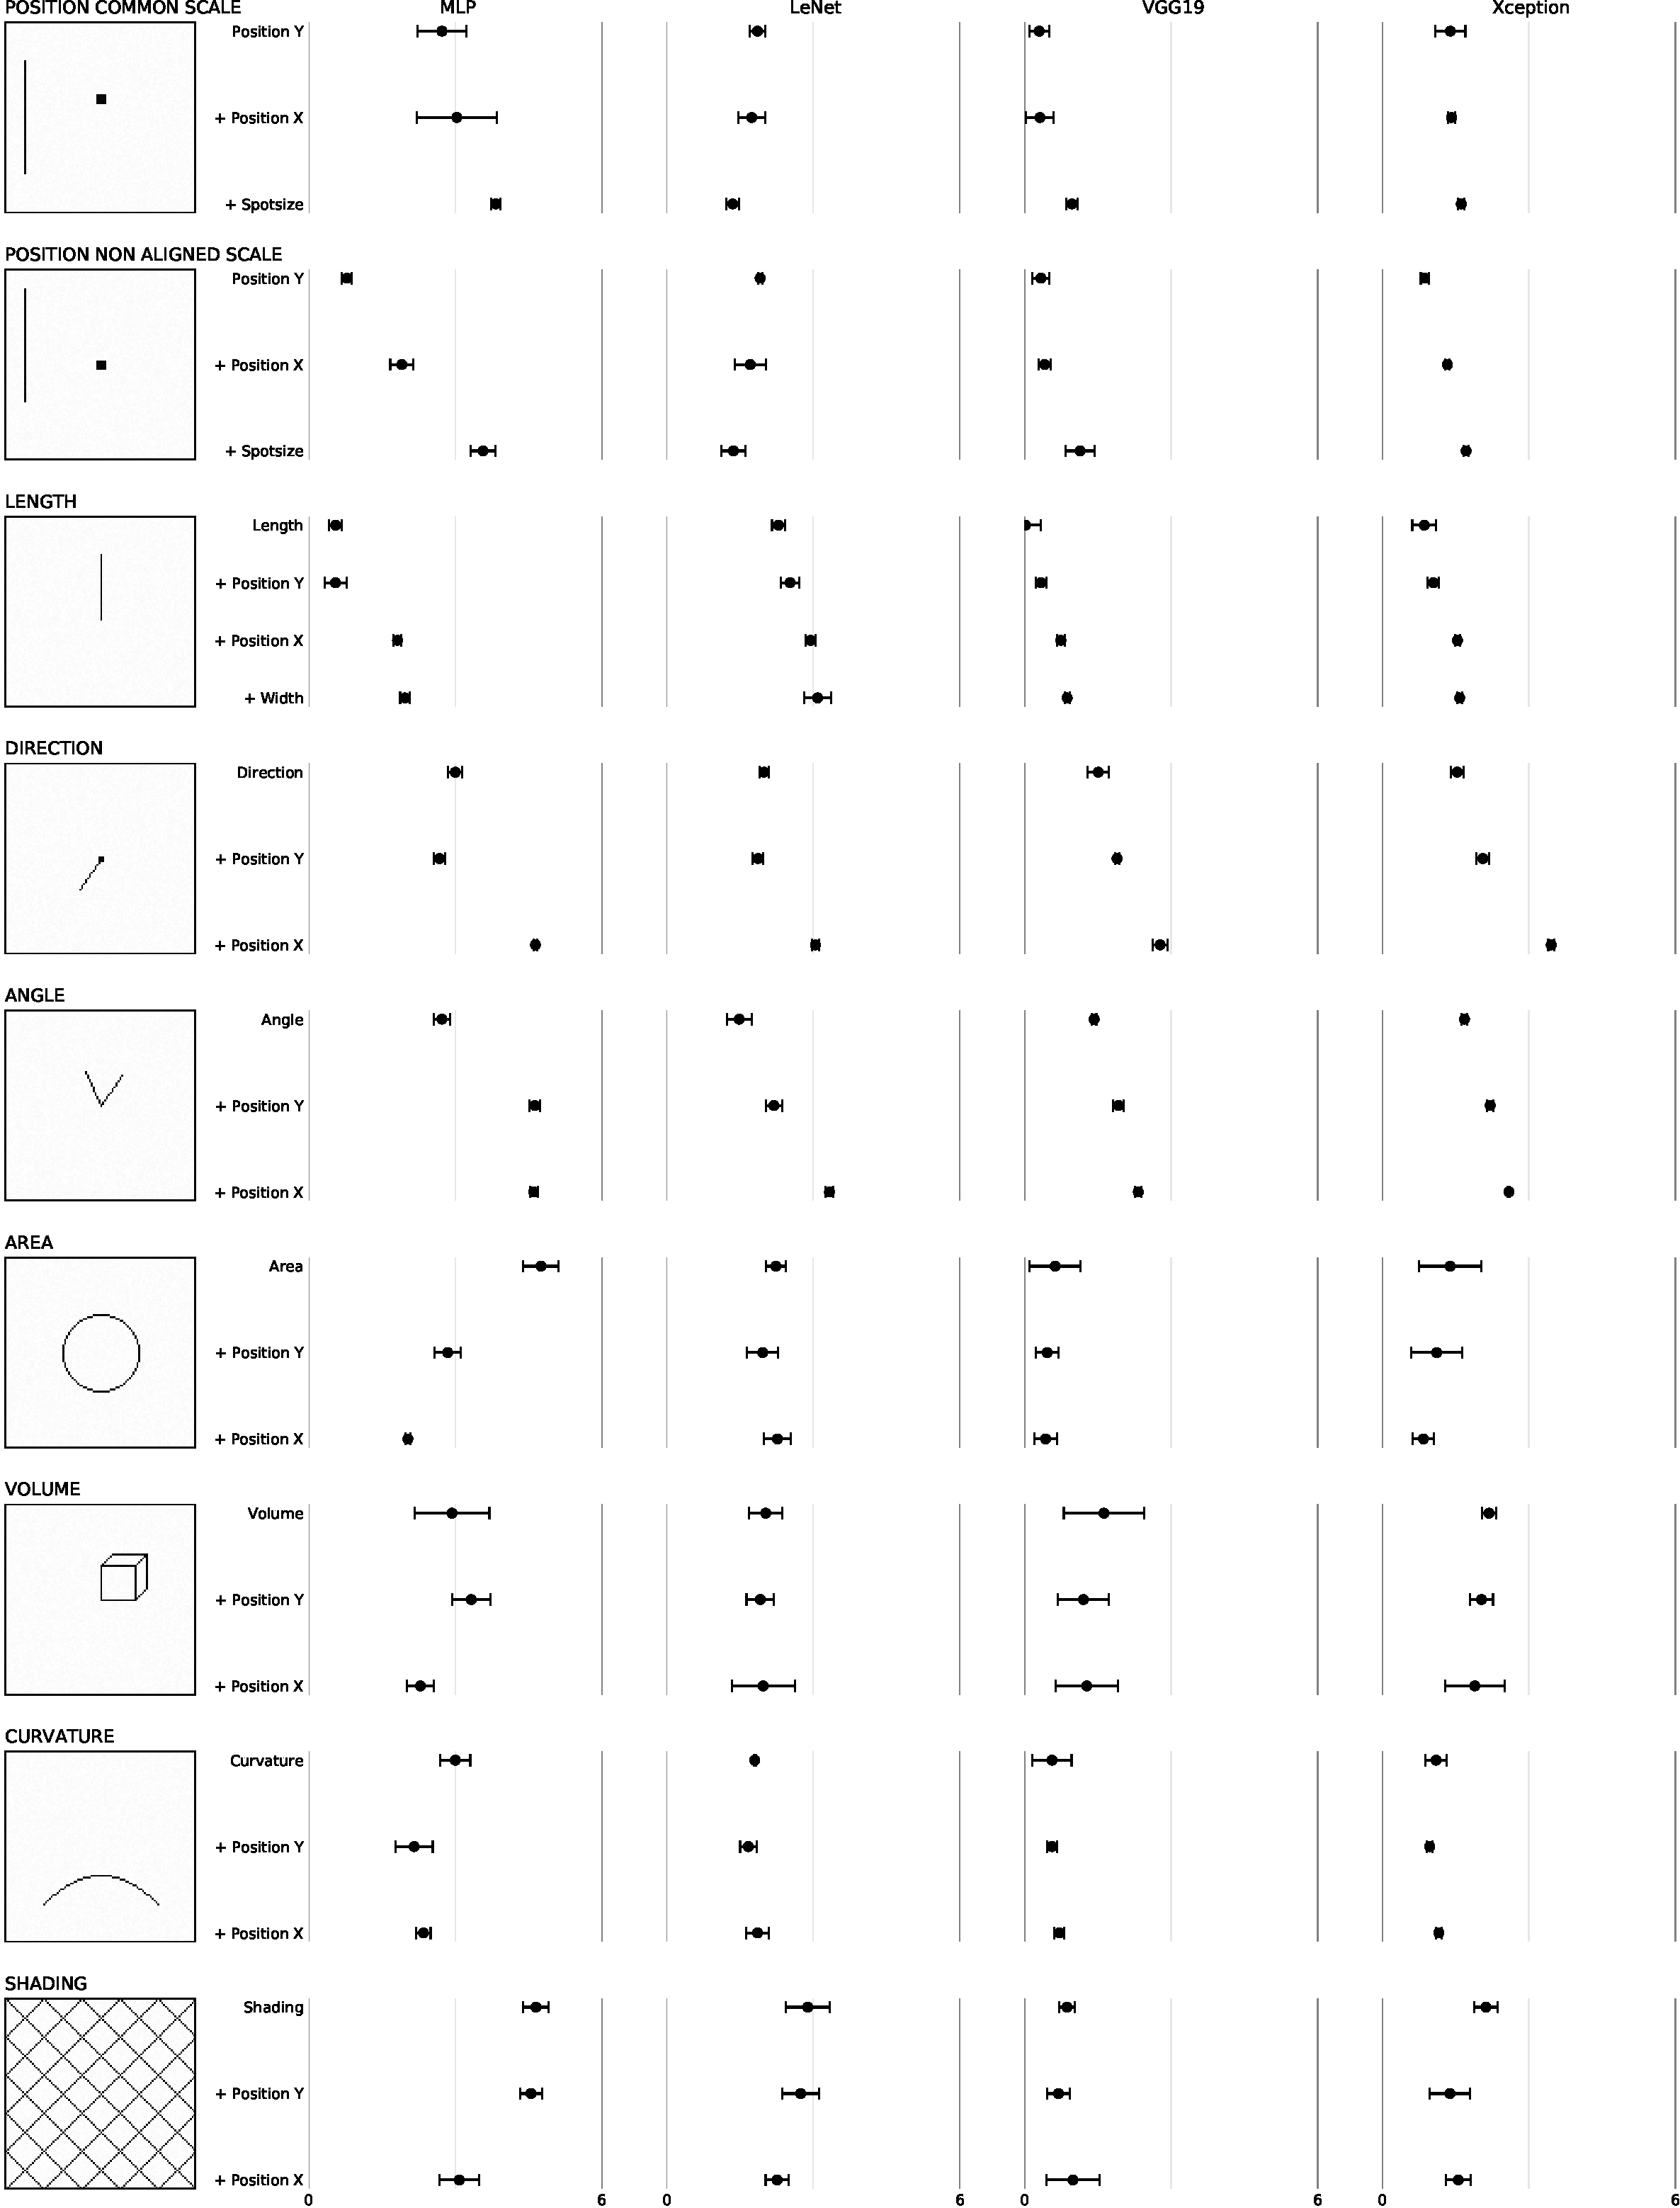
\includegraphics[width=\linewidth]{figure1.pdf}
  \caption{\textbf{Computational results of Elementary Perceptual Tasks experiment.} Log absolute error means and 95\% confidence intervals for computed perception of different classifiers on the \emph{elementary perceptual tasks} introduced by Cleveland and McGill 1984~\cite{cleveland_mcgill}. We test the performance of a Multi-layer Perceptron (MLP), the LeNet Convolutional Neural Network, as well as feature generation using the VGG19 and Xception networks trained on ImageNet.}
	\label{fig:figure1_results}
\end{figure*}

\textbf{Computational Perception Ranking.}

Cleveland McGills Ranking - can we observe something similar?

\begin{enumerate}
	\item Position along a common scale e.g. scatter plot
	\item Position on identical but nonaligned scales e.g. multiple scatter plots
	\item Length e.g. bar chart
	\item Angle \& Slope (tie) e.g. pie chart
	\item Area e.g. bubbles
	\item Volume, density, and color saturation (tie) e.g. heatmap
	\item Color hue e.g. newsmap
\end{enumerate}

\noindent{\textbf{Cross-classifier variability.}}

Can a neural network generalize on simple perceptual tasks?

\begin{figure}[t]
	  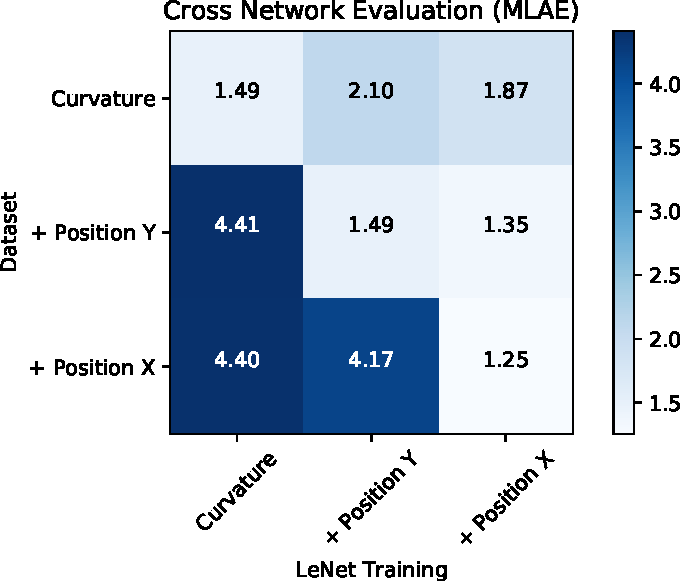
\includegraphics[width=\linewidth]{crossnetwork.pdf}
  \caption{\textbf{Cross-classifier variability for the perceptual task of measuring curvature.} We use predictions of LeNet classifiers trained on different parametrizations of the \emph{curvature} elementary perceptual task and measure the mean logistic absolute error (MLAE). The lower score, the better. Classifiers trained on curves with variable position can generalize even if the axis of translation varies. However, classifiers trained on fixed positions of curves are not able to measure translated curves.}
	\label{fig:cross_network}
\end{figure}


\subsection{Position-Angle Experiment}

Bar charts are more accurate (Fig.~\ref{fig:figure3_mlae}) and networks converge faster (Fig.~\ref{fig:figure3_val_loss}). This is great.

\begin{figure}[t]
	  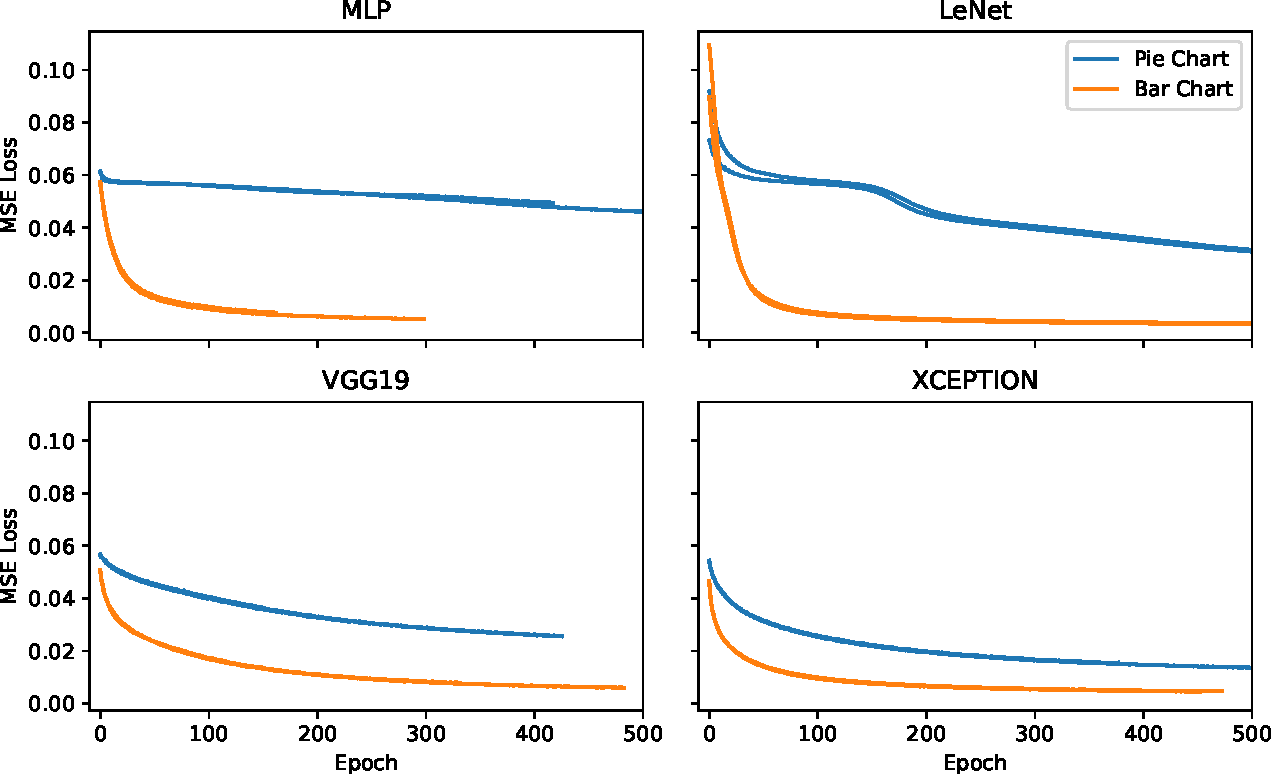
\includegraphics[width=\linewidth]{figure3_val_loss.pdf}
  \caption{\textbf{Classifier Efficiency of the Position-Angle experiment.} Mean Square Error (MSE) loss for the \emph{position-angle experiment} as described by Cleveland and McGill~\cite{cleveland_mcgill} which compares the visualization of pie charts and bar charts. We report the MSE measure for both encodings of four different classifier on previously unseen validation data.}
	\label{fig:figure3_val_loss}
\end{figure}

\begin{figure*}[t]
	  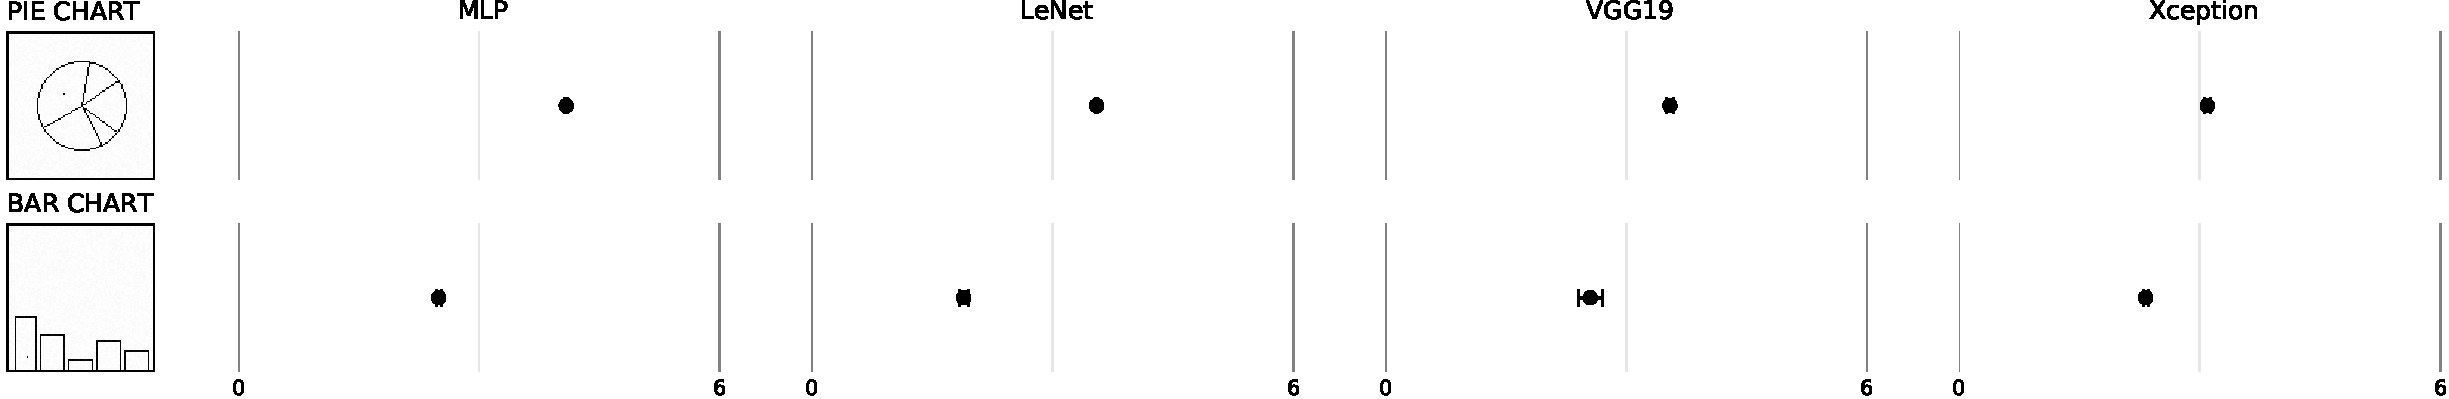
\includegraphics[width=\linewidth]{figure3_mlae.pdf}
  \caption{\textbf{Computational results of the Position-Angle experiment.} Log absolute error means and 95\% confidence intervals for the \emph{position-angle experiment} as described by Cleveland and McGill~\cite{cleveland_mcgill}. We test the performance of a Multi-layer Perceptron (MLP), the LeNet Convolutional Neural Network, as well as feature generation using the VGG19 and Xception networks trained on ImageNet.}
	\label{fig:figure3_mlae}
\end{figure*}

\subsection{Position-Length Experiment}

We have nothing yet here...


\subsection{Bars and Framed Rectangles Experiment}

First run indicates that framed rectangles perform better but we dont really know it yet.

\begin{figure}[t]
	  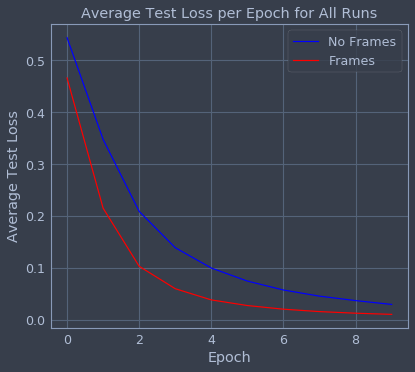
\includegraphics[width=\linewidth]{figure12_val_loss.png}
  \caption{\textbf{Classifier Efficiency of the Bars and Framed Rectangles experiment.} Categorical Cross-Entropy loss for the \emph{bars and framed rectangles experiment} as described by Cleveland and McGill~\cite{cleveland_mcgill}. The frame around the bars adds an additional visual cue enables faster network convergence. This is not yet reproducible!}
	\label{fig:figure12_val_loss}
\end{figure}
